\documentclass{report}
\usepackage{luatexja} % LuaTeXで日本語を使うためのパッケージ
\usepackage{luatexja-fontspec} % LuaTeX用の日本語フォント設定
% lualatex main && upmendex -r -c -s main.ist -g main && lualatex main  

% --- 数学関連 ---
\usepackage{amsmath, amssymb, amsfonts, mathtools, bm, amsthm} % 基本的な数学パッケージ
\usepackage{type1cm, upgreek} % 数式フォントとギリシャ文字k
\usepackage{physics, mhchem} % 物理や化学の記号や式の表記を簡単にする

% --- 表関連 ---
\usepackage{multirow, longtable, tabularx, array, colortbl, dcolumn, diagbox} % 表のレイアウトを柔軟にする
\usepackage{tablefootnote, truthtable} % 表中に注釈を追加、真理値表
\usepackage{tabularray} % 高度な表組みレイアウト

% --- グラフィック関連 ---
\usepackage{tikz, graphicx} % 図の描画と画像の挿入
% \usepackage{background} % ウォーターマークの設定
\usepackage{caption, subcaption} % 図や表のキャプション設定
\usepackage{float, here} % 図や表の位置指定

% --- レイアウトとページ設定 ---
\usepackage{fancyhdr} % ページヘッダー、フッター、余白の設定
\usepackage[top = 20truemm, bottom = 20truemm, left = 20truemm, right = 20truemm]{geometry}
\usepackage{fancybox, ascmac} % ボックスのデザイン

% --- 色とスタイル ---
\usepackage{xcolor, color, colortbl, tcolorbox, ulem} % 色とカラーボックス
\usepackage{listings, jvlisting} % コードの色付けとフォーマット
\definecolor{apsblue}{HTML}{2d3092}

% --- 参考文献関連 ---
% \usepackage[style=phys, backend=biber]{biblatex}
\usepackage[backend=biber, sortcites=true, style=phys, doi=false]{biblatex}
\usepackage{usebib} % 参考文献の管理と挿入
\usepackage{url} % URLとリンクの設定
\usepackage[colorlinks=true, linkcolor=apsblue, citecolor=apsblue, urlcolor=apsblue]{hyperref}

% --- その他の便利なパッケージ ---
\usepackage{footmisc} % 脚注のカスタマイズ
\usepackage{multicol} % 複数段組
\usepackage{comment} % コメントアウトの拡張
\usepackage{siunitx} % 単位の表記
\usepackage{docmute, needspace}
\usepackage{makeidx}

% \renewbibmacro*{title}{%
%   \printtext[title]{\printfield[titlecase]{title}.\addspace}%
% }
% --- 定理スタイルと数式設定 ---
\theoremstyle{definition} % 定義スタイル
\numberwithin{equation}{chapter} % 式番号をサブセクション単位でリセット

% --- その他の設定 ---
\allowdisplaybreaks % 数式の途中改ページ許可
\newcolumntype{t}{!{\vrule width 0.1pt}} % 新しいカラムタイプ
\newcolumntype{b}{!{\vrule width 1.5pt}} % 太いカラム
\UseTblrLibrary{amsmath, booktabs, counter, diagbox, functional, hook, html, nameref, siunitx, varwidth, zref} % tabularrayのライブラリ
\setlength{\columnseprule}{0.4pt} % カラム区切り線の太さ
% \captionsetup[figure]{font = bf} % 図のキャプションの太字設定
% \captionsetup[table]{font = bf} % 表のキャプションの太字設定
% \captionsetup[lstlisting]{font = bf} % コードのキャプションの太字設定
% \captionsetup[subfigure]{font = bf, labelformat = simple} % サブ図のキャプション設定
\setcounter{secnumdepth}{4} % セクションの深さ設定
\newcolumntype{d}{D{.}{.}{5}} % 数値のカラム
\newcolumntype{M}[1]{>{\centering\arraybackslash}m{#1}} % センター揃えのカラム
\DeclareMathOperator{\diag}{diag}
\everymath{\displaystyle} % 数式のスタイル

\setcounter{tocdepth}{0} % 目次の深さ
% \makeatletter
% \@addtoreset{equation}{chapter} % セクションごとに式番号をリセット
% \makeatother

\newcommand{\braketg}{\braket{\r{g}}}

% \DeclareFieldFormat{journal+issuetitle}{%
%   \iffieldundef{doi}
%     {\printfield{journal}%
%      \setunit*{\addspace}%
%      \printfield{volume}%
%      \setunit*{\addcomma\space}%
%      \printfield{pages}}
%     {\href{https://doi.org/\thefield{doi}}%
%      {\printfield{journal}%
%       \setunit*{\addspace}%
%       \printfield{volume}%
%       \setunit*{\addcomma\space}%
%       \printfield{pages}}}}

% \DeclareFieldFormat{year}{(\printfield{year})}
\DeclareSourcemap{
  \maps[datatype=bibtex, overwrite=true]{
    \map{
      \step[
        fieldsource=journal,
        match=\regexp{Physical\sReview\sLetters},
        replace={Phys. Rev. Lett.}
      ]
      \step[
        fieldsource=journal,
        match=\regexp{Physical\sReview\sA},
        replace={Phys. Rev. A}
      ]
      \step[
        fieldsource=journal,
        match=\regexp{Physical\sReview\sB},
        replace={Phys. Rev. B}
      ]
      \step[
        fieldsource=journal,
        match=\regexp{Physical\sReview\sC},
        replace={Phys. Rev. C}
      ]
      \step[
        fieldsource=journal,
        match=\regexp{Physical\sReview\sD},
        replace={Phys. Rev. D}
      ]
      \step[
        fieldsource=journal,
        match=\regexp{Physical\sReview\sE},
        replace={Phys. Rev. E}
      ]
      \step[
        fieldsource=journal,
        match=\regexp{Physical\sReview\sX},
        replace={Phys. Rev. X}
      ]
      \step[
        fieldsource=journal,
        match=\regexp{Reviews\sof\sModern\sPhysics},
        replace={Rev. Mod. Phys.}
      ]
      \step[
        fieldsource=journal,
        match=\regexp{Journal\sof\sApplied\sPhysics},
        replace={J. Appl. Phys.}
      ]
      \step[
        fieldsource=journal,
        match=\regexp{Applied\sPhysics\sA},
        replace={Appl. Phys. A}
      ]
      \step[
        fieldsource=journal,
        match=\regexp{Applied\sPhysics\sB},
        replace={Appl. Phys. B}
      ]
      \step[
        fieldsource=journal,
        match=\regexp{Applied\sPhysics\sLetters},
        replace={Appl. Phys. Lett.}
      ]
      \step[
        fieldsource=journal,
        match=\regexp{Review\sof\sScientific\sInstruments},
        replace={Rev. Sci. Instrum.}
      ]
      \step[
        fieldsource=journal,
        match=\regexp{Nature},
        replace={Nature}
      ]
      \step[
        fieldsource=journal,
        match=\regexp{Science},
        replace={Science}
      ]
      \step[
        fieldsource=journal,
        match=\regexp{Nature\sPhysics},
        replace={Nat. Phys.}
      ]
      \step[
        fieldsource=journal,
        match=\regexp{Nature\sCommunications},
        replace={Nat. Commun.}
      ]
      \step[
        fieldsource=journal,
        match=\regexp{Scientific\sReports},
        replace={Sci. Rep.}
      ]
      \step[
        fieldsource=journal,
        match=\regexp{Journal\sof\sPhysics\sA:\sMathematical\sand\sTheoretical},
        replace={J. Phys. A: Math. Theor.}
      ]
      \step[
        fieldsource=journal,
        match=\regexp{Journal\sof\sPhysics\sB:\sAtomic,\sMolecular\sand\sOptical\sPhysics},
        replace={J. Phys. B: At. Mol. Opt. Phys.}
      ]
      \step[
        fieldsource=journal,
        match=\regexp{Journal\sof\sPhysics:\sCondensed\sMatter},
        replace={J. Phys.: Condens. Matter}
      ]
      \step[
        fieldsource=journal,
        match=\regexp{Annalen\sder\sPhysik},
        replace={Ann. Phys.}
      ]
      \step[
        fieldsource=journal,
        match=\regexp{Europhysics\sLetters},
        replace={Europhys. Lett.}
      ]
      \step[
        fieldsource=journal,
        match=\regexp{New\sJournal\sof\sPhysics},
        replace={New J. Phys.}
      ]
      \step[
        fieldsource=journal,
        match=\regexp{Physics\sLetters\sA},
        replace={Phys. Lett. A}
      ]
      \step[
          fieldsource=journal,
          match=\regexp{Physics\sLetters\sB},
          replace={Phys. Lett. B}
      ]
      \step[
          fieldsource=journal,
          match=\regexp{Optical\sand\sQuantum\sElectronics},
          replace={Opt. Quantum Electron.}
      ]
    }
  }
}
\newcommand{\inner}[2]{\left\langle #1, #2 \right\rangle}
\renewcommand{\figurename}{図}
\renewcommand{\i}{\mathrm{i}} % 複素数単位i
\renewcommand{\laplacian}{\grad^2} % ラプラシアンの記号
\renewcommand{\thesubfigure}{(\alph{subfigure})} % サブ図の番号形式
\newcommand{\m}[3]{\multicolumn{#1}{#2}{#3}} % マルチカラムのショートカット
\renewcommand{\r}[1]{\mathrm{#1}} % mathrmのショートカット
\newcommand{\e}{\mathrm{e}} % 自然対数の底e
\newcommand{\Ef}{E_{\mathrm{F}}} % フェルミエネルギー
\renewcommand{\c}{\si{\degreeCelsius}} % 摂氏記号
\renewcommand{\d}{\r{d}} % d記号
\renewcommand{\t}[1]{\texttt{#1}} % タイプライタフォント
\newcommand{\kb}{k_{\mathrm{B}}} % ボルツマン定数
\renewcommand{\epsilon}{\varepsilon}
\newcommand{\fullref}[1]{\textbf{\ref{#1} \nameref{#1}}}
\newcommand{\reff}[1]{{図\ref{#1}}} % 図参照のショートカット
\newcommand{\reft}[1]{{表\ref{#1}}} % 表参照のショートカット
\newcommand{\refe}[1]{{式\eqref{#1}}} % 式参照のショートカット
\newcommand{\refp}[1]{{コード\ref{#1}}} % コード参照のショートカット
\renewcommand{\lstlistingname}{コード} % コードリストの名前
\renewcommand{\theequation}{\thesection.\arabic{equation}} % 式番号の形式
\renewcommand{\footrulewidth}{0.4pt} % フッターの線
\newcommand{\mar}[1]{\textcircled{\scriptsize #1}} % 丸囲み文字
\newcommand{\combination}[2]{{}_{#1} \mathrm{C}_{#2}} % 組み合わせ
\newcommand{\thline}{\noalign{\hrule height 0.1pt}} % 細い横線
\newcommand{\bhline}{\noalign{\hrule height 1.5pt}} % 太い横線
\renewcommand{\appendixname}{付録}

\ExecuteBibliographyOptions{
  sorting=none, biblabel=brackets, articletitle=true, chaptertitle=false,
  pageranges=false, maxnames=99, minnames=1, hyperref=auto, abbreviate=true
}
\bibliography{ref.bib}

% \DeclareFieldFormat{eprint}{arXiv:\href{http://arxiv.org/abs/#1}{#1}}
% \DeclareFieldFormat{eprint}{arXiv:\href{http://arxiv.org/abs/ #1}{#1} (\thefield{year})}
% 出力のカスタマイズ(タイトルを省略し、arXiv形式を適用)
% \DeclareFieldFormat[article]{title}{\mkbibemph{#1}}  % 必要に応じて
% \AtEveryBibitem{\clearfield{doi}}  % DOIフィールドを消す
% \AtEveryBibitem{\clearfield{url}}  % URLフィールドを消す
% \DeclareFieldFormat[article]{note}{\mkbibparens{arXiv:#1}}  % arXivの表示形式を調整
% \AtEveryBibitem{
%   \clearfield{title}
% }
% --- メタ情報 ---
\title{論文まとめノート}
\date{更新日: \today}
\author{Haruki AOKI}

\begin{document}
  \maketitle
  \tableofcontents
  \chapter{Input and output in damped quantum systems: Quantum stochastic differential equations and the master equation}
    \begin{boxnote}
      \begin{description}
        \item[種類] Article
        \item[閲覧日] 13th May 2025
        \item[キーワード] 
        \item[文献番号] \cite{PhysRevA.31.3761}
        \item[関連論文] 特になし.
      \end{description}
    \end{boxnote}
    \section{量子Langevin方程式}
      着目系$\hat{H}_{\r{sys}}$,熱浴$\hat{H}_{\r{B}}$,それらの相互作用$\hat{H}_{\r{int}}$の全体を考える.
      全体のハミルトニアンは,
      \begin{align}
        \hat{H} = \hat{H}_{\r{sys}} + \hat{H}_{\r{B}} + \hat{H}_{\r{int}}
      \end{align}
      である.
      熱浴はBoson場であるとして,熱浴のハミルトニアンと相互作用のハミルトニアンは,
      \begin{align}
        \hat{H}_{\r{B}}(t) &\coloneqq \int_{-\infty}^{\infty}\dd{\omega} \hbar\omega \hat{b}^{\dag}(\omega, t)\hat{b}(\omega, t) \\ 
        \hat{H}_{\r{int}}(t) &\coloneqq \int_{-\infty}^{\infty}\dd{\omega} \hbar\i\kappa(\omega)\qty(\hat{b}^{\dag}(\omega, t)\hat{c}(t) - \hat{c}^{\dag}(t)\hat{b}(\omega, t))
      \end{align}
      とする.
      $\hat{b}(\omega, t)$は時刻$t$における,周波数モード$\omega$の消滅演算子であり,
      \begin{align}
        \qty[\hat{b}(\omega, t), \hat{b}^{\dag}(\omega', t)] = \delta(\omega - \omega')\quad \qty[\hat{b}(\omega, t), \hat{b}(\omega', t)] = 0
      \end{align}
      であるとする.
      また,$\hat{c}$は着目系の演算子のうち,熱浴と相互作用するものである.
      さて,熱浴の演算子$\hat{b}(\omega, t)$や,着目系の任意の物理量$\hat{a}(t)$の時間発展を考えよう.
      Heisenbergの方程式より,
      \begin{align}
        \pdv{\hat{b}}{t}(\omega, t) =& -\frac{\i}{\hbar}\qty[\hat{b}(\omega, t), \hat{H}(t)] \\ 
        =& -\frac{\i}{\hbar}\qty[\hat{b}(\omega, t), \hat{H}_{\r{B}}(t)] - \frac{\i}{\hbar}\qty[\hat{b}(\omega, t), \hat{H}_{\r{int}}(t)] \\ 
        =& -\frac{\i}{\hbar}\int_{-\infty}^{\infty}\dd{\omega'} \hbar\omega'\qty(\hat{b}(\omega, t)\hat{b}^{\dag}(\omega', t)\hat{b}(\omega', t) - \hat{b}^{\dag}(\omega', t)\hat{b}(\omega', t)\hat{b}(\omega, t)) \\ 
        &- \frac{\i}{\hbar}\int_{-\infty}^{\infty}\dd{\omega'} \hbar\i\kappa(\omega')\qty(\hat{b}(\omega, t)\hat{b}^{\dag}(\omega', t)\hat{c}(t) - \hat{b}^{\dag}(\omega', t)\hat{c}(t)\hat{b}(\omega, t)) \\ 
        =& -\i\omega\hat{b}(\omega, t) + \kappa(\omega)\hat{c}(t) \\ 
        \dv{\hat{a}}{t}(t) =& -\frac{\i}{\hbar}\qty[\hat{b}(\omega, t), \hat{H}(t)] \\ 
        =& -\frac{\i}{\hbar}\qty[\hat{a}(t), \hat{H}_{\r{sys}}(t)] - \frac{\i}{\hbar}\qty[\hat{a}(t), \hat{H}_{\r{int}}(t)] \\ 
        =& -\frac{\i}{\hbar}\qty[\hat{a}(t), \hat{H}_{\r{sys}}(t)] + \int_{-\infty}^{\infty}\kappa(\omega)\qty(\hat{b}^{\dag}(\omega, t)\qty[\hat{a}(t), \hat{c}(t)] - \qty[\hat{a}(t), \hat{c}^{\dag}(t)]\hat{b}(\omega, t))
      \end{align}
      である.
      まず,$\hat{b}(\omega, t)$に関する非斉次微分方程式,
      \begin{align}
        \pdv{\hat{b}}{t}(\omega, t) =& -\i\omega\hat{b}(\omega, t) + \kappa(\omega)\hat{c}(t)
      \end{align}
      を未定係数法で解く.
      斉次式は,
      \begin{align}
        \pdv{\hat{b}}{t}(\omega, t) = -\i\omega\hat{b}(\omega, t)
      \end{align}
      であるので,斉次解は,
      \begin{align}
        \hat{b}(\omega, t) = \e^{-\i\omega(t - t_0)}\hat{b}_0(\omega),\quad \hat{b}_0(\omega) \coloneqq \hat{b}(\omega, t_0)
      \end{align}
      である.
      未定係数法では,時間に依存しない$\hat{b}_0(\omega)$を時間依存する項とみなして,元の微分方程式に代入するのであった.
      すると,
      \begin{align}
        \e^{-\i\omega(t - t_0)}\pdv{\hat{b}_0}{t} (\omega, t) - \i\omega(t - t_0)\e^{-\i\omega(t - t_0)}\hat{b}_0(\omega, t) =& -\i\omega\e^{-\i\omega(t - t_0)}\hat{b}_0(\omega) + \kappa(\omega)\hat{c}(t) \\ 
        \iff \pdv{\hat{b}_0}{t} (\omega, t) =& \kappa(\omega)\e^{\i\omega(t - t_0)}\hat{c}(t) \\ 
        \implies \hat{b}_0(\omega, t) =& \kappa(\omega)\int_{t_0}^{t}\dd{t'}\e^{\i\omega(t' - t_0)}\hat{c}(t')
      \end{align}
      と書ける.
      よって,
      \begin{align}
        \hat{b}(\omega, t) =& \e^{-\i\omega(t - t_0)}\hat{b}_0(\omega) + \e^{-\i\omega(t - t_0)}\kappa(\omega)\int_{t_0}^{t}\dd{t'}\e^{\i\omega(t' - t_0)}\hat{c}(t') \\ 
        \iff \hat{b}(\omega, t) =& \e^{-\i\omega(t - t_0)}\hat{b}_0(\omega) + \kappa(\omega)\int_{t_0}^{t}\dd{t'}\e^{-\i\omega(t - t')}\hat{c}(t') \label{PhysRevA.31.3761-b-simple-representation}
      \end{align}
      である.
      $\hat{a}(t)$に関する微分方程式は,\refe{PhysRevA.31.3761-b-simple-representation}を用いて,
      \begin{align}
        \dv{\hat{a}}{t}(t) = -\frac{\i}{\hbar}\qty[\hat{a}(t), \hat{H}_{\r{sys}}(t)] &+ \int_{-\infty}^{\infty}\dd{\omega}\kappa(\omega)\qty{\e^{\i\omega(t - t_0)}\hat{b}^{\dag}_0(\omega)\qty[\hat{a}(t), \hat{c}(t)] - \e^{-\i\omega(t - t_0)}\qty[\hat{a}(t), \hat{c}^{\dag}(t)]\hat{b}_0(\omega)} \\ 
        &+ \int_{-\infty}^{\infty}\dd{\omega}\qty[\kappa(\omega)]^2\int_{t_0}^{t}\dd{t'}\qty(\e^{\i\omega(t - t')}\hat{c}^{\dag}(t')\qty[\hat{a}(t), \hat{c}(t)] - \qty[\hat{a}(t), \hat{c}^{\dag}(t)]\e^{-\i\omega(t - t')}\hat{c}(t')) \label{PhysRevA.31.3761-a-pdv}
      \end{align}
      となる.
      \par
      \refe{PhysRevA.31.3761-a-pdv}に第1 Markov近似を行う.
      すなわち,
      \begin{align}
        \kappa(\omega) = \sqrt{\frac{\gamma}{2\pi}}
      \end{align}
      とする.
      \par
      ところで,$1$をFourier変換すると,
      \begin{align}
        \int_{-\infty}^{\infty}\dd{\omega}\e^{-\i\omega(t - t')} = 2\pi\delta(t - t')
      \end{align}
      となる.
      また,デルタ函数は偶函数であるから,
      \begin{align}
        \int_{t_0}^{t}\dd{t'}c(t')\delta(t - t') =& \int_{0}^{t - t_0}\dd{\tau}c(t - \tau)\delta(\tau) \\ 
        =& \int_{0}^{\infty}\dd{\tau}\delta(t - \tau)\delta(\tau) \\ 
        =& \frac{1}{2}\int_{-\infty}^{\infty}\dd{\tau}\delta(t - \tau)\delta(\tau) \\ 
        =& \frac{1}{2}c(t)
      \end{align}
      となる.
      また,初期状態での熱浴の演算子$\hat{b}_0(\omega) = \hat{b}(\omega, 0)$のFourier変換を,
      \begin{align}
        \hat{b}_{\r{in}}(t) \coloneqq \frac{1}{\sqrt{2\pi}}\int_{-\infty}^{\infty}\dd{\omega}\e^{-\i\omega(t - t_0)}\hat{b}_0
      \end{align}
      と定義する.
      これらの記法を用いると\refe{PhysRevA.31.3761-a-pdv}は,
      \begin{align}
        \dv{\hat{a}}{t}(t) =& -\frac{\i}{\hbar}\qty[\hat{a}(t), \hat{H}_{\r{sys}}(t)] + \int_{-\infty}^{\infty}\dd{\omega}\kappa(\omega)\qty{\e^{\i\omega(t - t_0)}\hat{b}^{\dag}_0(\omega)\qty[\hat{a}(t), \hat{c}(t)] - \e^{-\i\omega(t - t_0)}\qty[\hat{a}(t), \hat{c}^{\dag}(t)]\hat{b}_0(\omega)} \\ 
        &+ \int_{-\infty}^{\infty}\dd{\omega}\qty[\kappa(\omega)]^2\int_{t_0}^{t}\dd{t'}\qty(\e^{\i\omega(t - t')}\hat{c}^{\dag}(t')\qty[\hat{a}(t), \hat{c}(t)] - \qty[\hat{a}(t), \hat{c}^{\dag}(t)]\e^{-\i\omega(t - t')}\hat{c}(t')) \\ 
        =& -\frac{\i}{\hbar}\qty[\hat{a}(t), \hat{H}_{\r{sys}}(t)] + \sqrt{\frac{\gamma}{2\pi}}\qty[\qty{\int_{-\infty}^{\infty}\dd{\omega}\e^{\i\omega(t - t_0)}\hat{b}^{\dag}_0}\qty[\hat{a}(t), \hat{c}(t)] - \qty[\hat{a}(t), \hat{c}^{\dag}(t)]\qty{\int_{-\infty}^{\infty}\dd{\omega}\e^{-\i\omega(t - t_0)}\hat{b}^{\dag}_0}] \\ 
        &+ \frac{\gamma}{2\pi}\qty[\int_{t_0}^{t}\dd{t'}\qty{\int_{-\infty}^{\infty}\dd{\omega}\e^{\i\omega(t - t')}}\hat{c}^{\dag}(t')\qty[\hat{a}(t), \hat{c}(t)] - \int_{t_0}^{t}\dd{t'}\qty{\int_{-\infty}^{\infty}\dd{\omega}\e^{-\i\omega(t - t')}}\qty[\hat{a}(t), \hat{c}(t)]\hat{c}(t')] \\ 
        =& -\frac{\i}{\hbar}\qty[\hat{a}(t), \hat{H}_{\r{sys}}(t)] + \sqrt{\gamma}\qty[\hat{b}_{\r{in}}(t)\qty[\hat{a}(t), \hat{c}(t)] - \qty[\hat{a}(t), \hat{c}^{\dag}(t)]\hat{b}^{\dag}_{\r{in}}(t)] \\ 
        &+ \gamma\qty[\int_{t_0}^{t}\dd{t'}\delta(t - t')\hat{c}^{\dag}(t')\qty[\hat{a}(t), \hat{c}(t)] - \int_{t_0}^{t}\dd{t'}\delta(t - t')\qty[\hat{a}(t), \hat{c}(t)]\hat{c}(t')] \\ 
        =& -\frac{\i}{\hbar}\qty[\hat{a}(t), \hat{H}_{\r{sys}}(t)] + \sqrt{\gamma}\hat{b}_{\r{in}}(t)\qty[\hat{a}(t), \hat{c}(t)] - \sqrt{\gamma}\qty[\hat{a}(t), \hat{c}^{\dag}(t)]\hat{b}^{\dag}_{\r{in}}(t) + \frac{\gamma}{2}\hat{c}^{\dag}(t)\qty[\hat{a}(t), \hat{c}(t)] - \frac{\gamma}{2}\qty[\hat{a}(t), \hat{c}(t)]\hat{c}(t) \\ 
        =& -\frac{\i}{\hbar}\qty[\hat{a}(t), \hat{H}_{\r{sys}}(t)] - \qty[\hat{a}(t), \hat{c}^{\dag}(t)]\qty(\sqrt{\gamma}\hat{b}_{\r{in}} + \frac{\gamma}{2}\hat{c}) + \qty(\sqrt{\gamma}\hat{b}^{\dag}_{\r{in}} + \frac{\gamma}{2}\hat{c}^{\dag})\qty[\hat{a}(t), \hat{c}(t)] 
      \end{align}
      となる.
      よって,$\hat{a}(t)$の時間発展は,
      \begin{align}
        \dv{a}{t} = -\frac{\i}{\hbar}\qty[\hat{a}(t), \hat{H}_{\r{sys}}(t)] - \qty[\hat{a}(t), \hat{c}^{\dag}(t)]\qty(\sqrt{\gamma}\hat{b}_{\r{in}}(t) + \frac{\gamma}{2}\hat{c}(t)) + \qty(\sqrt{\gamma}\hat{b}^{\dag}_{\r{in}}(t) + \frac{\gamma}{2}\hat{c}^{\dag}(t))\qty[\hat{a}(t), \hat{c}(t)] \label{PhysRevA.31.3761-a-markov-approximated}
      \end{align}
      と書ける.
      \par
      第1 Markov近似を行った\refe{PhysRevA.31.3761-a-pdv}は次の4つの特徴を持つ.
      \begin{enumerate}
        \item 着目系に関して減衰項が存在する.
          着目系が調和振動子モデルのハミルトニアンを持ち,その周波数は$\omega_0$の整数倍であるとする.
          熱浴と相互作用する着目系の演算子は$\hat{a}$であり,またそれだけのとき$\hat{c}(t) = \hat{a}(t)$として\refe{PhysRevA.31.3761-a-markov-approximated}は,
          \begin{align}
            \dv{a}{t} =& -\frac{\i}{\hbar}\qty[\hat{a}(t), \hbar\omega_0\hat{a}^{\dag}(t)\hat{a}(t)] - \qty[\hat{a}(t), \hat{a}^{\dag}(t)]\qty(\sqrt{\gamma}\hat{b}_{\r{in}}(t) + \frac{\gamma}{2}\hat{a}(t)) + \qty(\sqrt{\gamma}\hat{b}^{\dag}_{\r{in}}(t) + \frac{\gamma}{2}\hat{a}^{\dag}(t))\qty[\hat{a}(t), \hat{a}(t)] \\ 
            \iff \dv{a}{t} =& -\frac{\i}{\hbar}\hat{a}(t) - \sqrt{\gamma}\hat{b}_{\r{in}}(t) - \frac{\gamma}{2}\hat{a}(t)
          \end{align}
          となり,第1項は周波数$\hat{\omega}_0$で振動する項,第2項は減衰する項である.
        \item $\hat{b}_\r{in}$はノイズ項である.
          初期状態$\hat{b}_{\r{in}}$に依存せず,\refe{PhysRevA.31.3761-a-pdv}は成立する.
      \end{enumerate}
      伊藤積分以降,わからない.
      数理物理の分野になるから深追いしないことにした.
  \chapter{Realization of Quantum Toffoli Gate with Trapped Ions}
    \begin{boxnote}
        \begin{description}
          \item[種類] Article
          \item[閲覧日] 14th May 2025
          \item[キーワード] Trapped-ion, Toffoli gate, Quantum Computer
          \item[文献番号] \cite{PhysRevA.106.042603}
          \item[関連論文] \cite{schmidt2003realize}, \cite{schmidt2003realization}
        \end{description}
      \end{boxnote}
  \chapter{Coherent control of a local phonon in trapped ions using dynamical decoupling}
    \begin{boxnote}
      \begin{description}
        \item[種類] Article
        \item[閲覧日] 14th May 2025
        \item[キーワード] Trapped-ion, Dynamical decoupling
        \item[文献番号] \cite{PhysRevA.106.042603}
        \item[関連論文] Quditへの応用\cite{PhysRevA.109.022620}, 論文の元のアイデア\cite{PhysRevLett.112.050504}
      \end{description}
    \end{boxnote}
    \section{行ったこと}
      ダイナミカルデカップリングを用いて,ホッピングによる状態遷移から量子ビットを守る.
    \section{モチベーション}
      イオントラップ系は,イオンの内部状態の2準位系とボゾン的な運動状態が結合した系である.
      そのうち,運動状態を用いた量子計算であるボゾンサンプリングが量子コンピュータの1つとして注目されている.
      ボゾンサンプリングは,$\# P$困難問題の1つであるSlater行列式を計算することに期待されている.
      イオンを線状に並べて計算を行う方式では,イオンの運動状態がCoulomb力によって相互作用をする.
      そのハミルトニアンは,
      \begin{align}
        \hat{H}_{\r{hop}} = \frac{\kappa_{12}}{2}\qty(\hat{a}_1\hat{a}^{\dag}_2 + \hat{a}^{\dag}_1\hat{a}_2)
      \end{align}
      である.
      このホッピングによって系の状態が変わってしまうことを,パルスを打って時間反転することで打ち消そうとすることが今回のモチベーションである.
  \chapter{Cavity-Enhance Solid-state Nuclear Spin Gyroscope}
    \begin{boxnote}
      \begin{description}
        \item[種類] Article
        \item[閲覧日] 17th May 2025
        \item[キーワード] Nitrogen Vacancy, Cavity QED
        \item[文献番号] \cite{PhysRevLett.134.183603}
        \item[関連論文] 核スピンを用いた角速度センシング\cite{PhysRevA.86.062104},核スピンと電子スピンを用いた角速度の保存\cite{wang2024spin}
      \end{description}
    \end{boxnote}
    \section{行ったこと}
      \begin{enumerate}
        \item 反転分布なしのメーザをnNV-cQED系で実現.
        \item NVの電子スピン-核スピン-共振器系を用いた,NVを用いた角速度センシングの精度の3桁改善.
        \item 角速度のベクトルセンシング.
        \item 核スピンの環境系によるノイズを影響を電子スピンで補正する共磁力計の実現.
      \end{enumerate}
    \section{詳細}
      \subsection{ドライブ・プローブ干渉}
        NVの電子スピン-核スピン系のハミルトニアンは,
        \begin{align}
          \hat{H}_{\r{NV}} = D\hat{S}^2_z + \gamma_{\r{e}}\hat{\bm{S}}\cdot\bm{B} + Q\hat{I}^2_z - \gamma_{\r{n}}\hat{\bm{I}}\cdot\bm{B} + \hat{\bm{S}}\mathcal{A}\hat{\bm{I}}
        \end{align}
        と書ける.
        ただし,$\hat{S}_z$は電子スピンの演算子,$\hat{I}_z$は核スピンの演算子,$\mathcal{A}$は対角的な超微細構造のテンソルである.
        どちらもスピン1系であり,$\ket{1} \coloneqq \ket{m_{\r{s}} = 0, m_{\r{I}} = -1}$,$\ket{2} \coloneqq \ket{m_{\r{s}} = 0, m_{\r{I}} = 0}$,$\ket{\r{e}} \coloneqq \ket{m_{\r{s}} = 1, m_{\r{I}} = -1}$のような
        \Lambda 型準位として用いる.
        \begin{figure}[H]
          \centering
          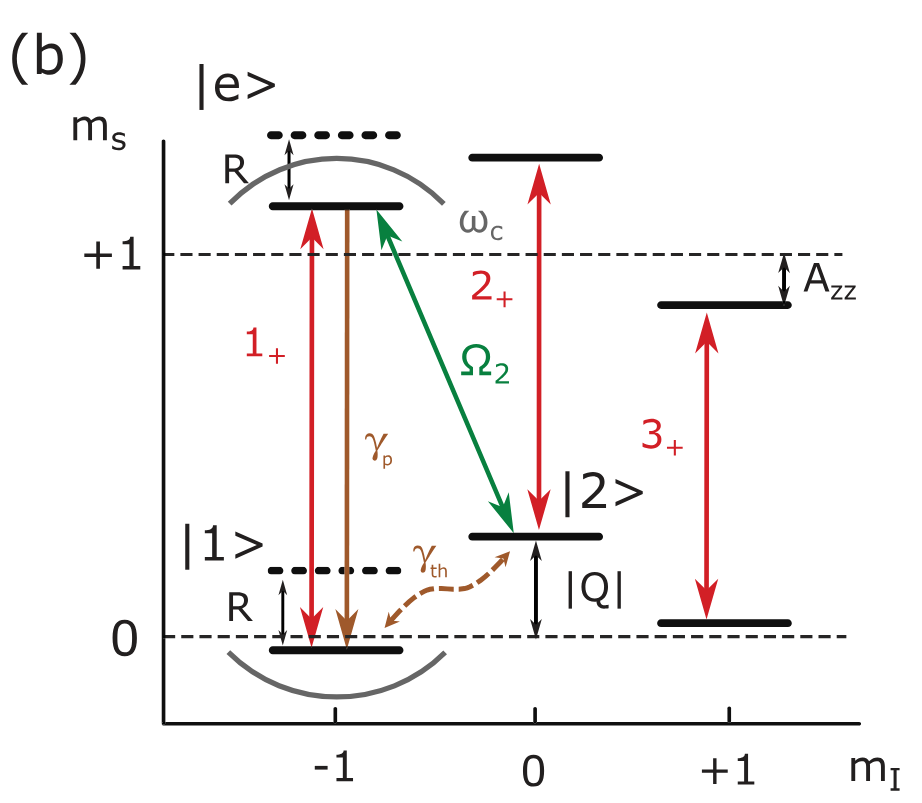
\includegraphics[width = 0.5\linewidth]{./src/Cavity-Enhanced_Solid-State_Nuclear_Spin_Gyroscope/1_b.png}
          \caption{
            今回用いるNVの準位図.
            横軸が核スピン,縦軸が電子スピンを表している.
          }
        \end{figure}
        $N$個のNVが集まったアンサンブルを考える.
        プローブとして,共振器(マイクロ波)のモード$\hat{a}$は,エネルギー差が$\omega_{\r{c}}$である$\ket{1}$と$\ket{\r{e}}$と結合しているとする
        また$\ket{2}$と$\ket{\r{e}}$を遷移するRabi周波数が$\Omega_2$となるように周波数$\omega_{\r{d}}$のドライブ光が入っているとする.
        共振器の結合$g$が共振器の緩和レート$\kappa$や電子スピンのデコヒーレンスレート$\Gamma$よりも十分大きい,$C = 4g^2 / (\kappa\Gamma) \sim 20$の強結合領域を考える.
        $\omega_{\r{c}}$と$\omega_{\r{d}}$の離調$\Delta$が0になると,電磁誘導透過(EIT)が起こる.
        \begin{figure}[H]
          \centering
          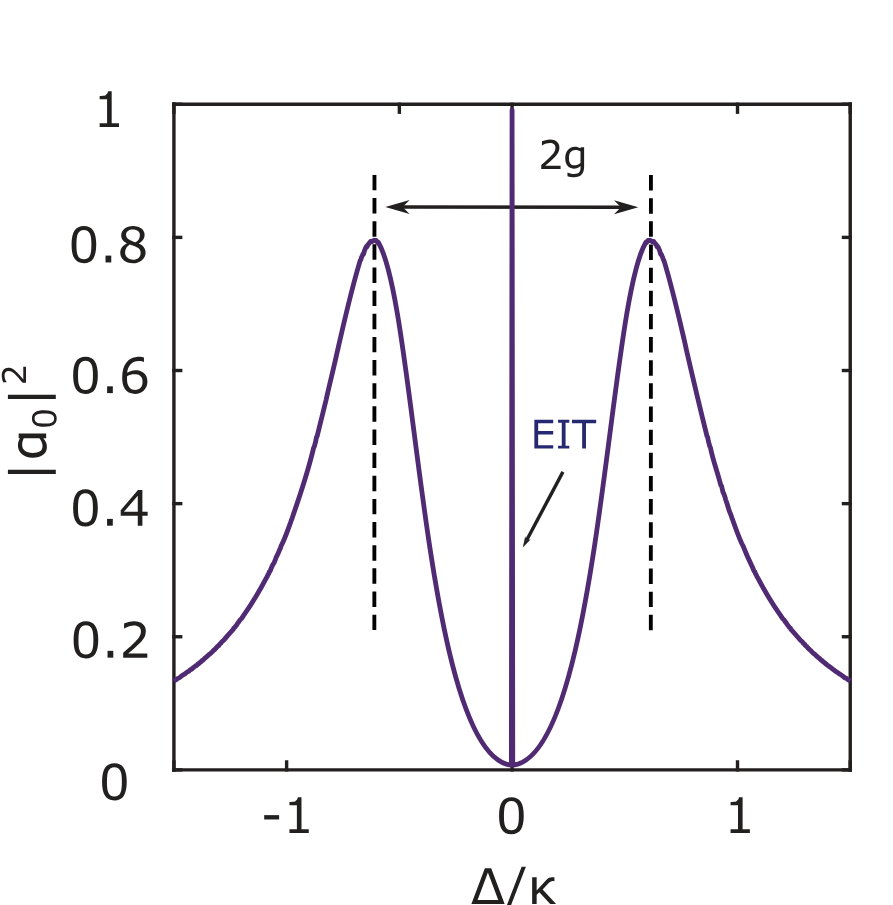
\includegraphics[width = 0.5\linewidth]{./src/Cavity-Enhanced_Solid-State_Nuclear_Spin_Gyroscope/1_d.png}
          \caption{EITの様子.$\abs{\alpha}_0$がNVセンターの吸収強度を表す.この現象は2つの場の量子干渉ととらえることができる.}
        \end{figure}
        さらにRabi周波数を大きくすると,透過するだけでなく,プローブ光が増強されること(MWI)が分かる.
        \begin{figure}[H]
          \centering
          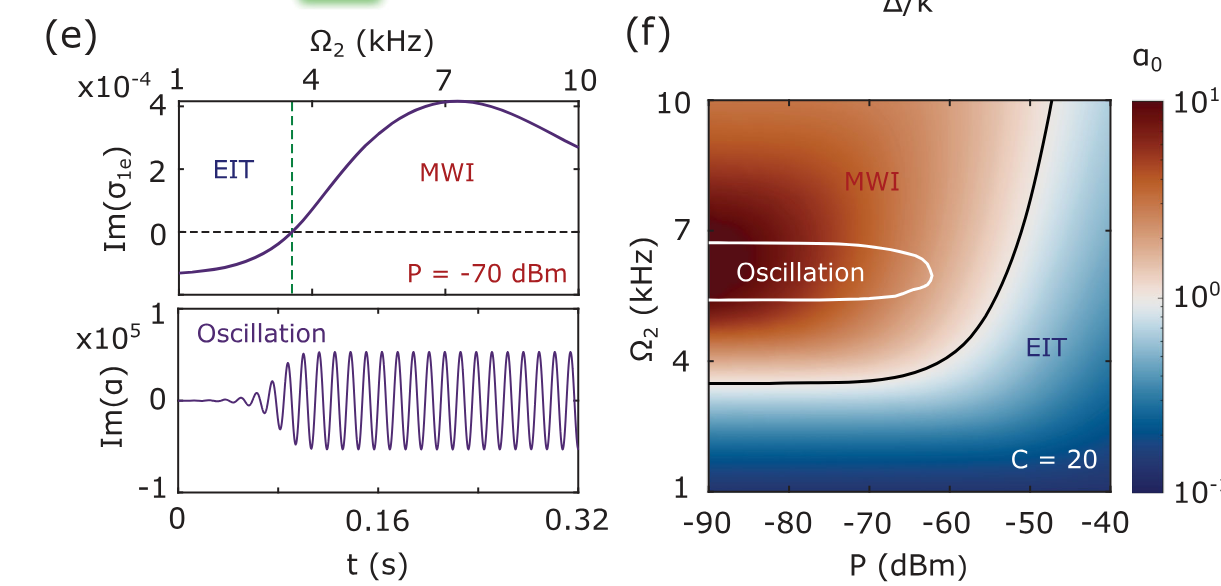
\includegraphics[width = 0.5\linewidth]{./src/Cavity-Enhanced_Solid-State_Nuclear_Spin_Gyroscope/1_e_d.png}
          \caption{(e): Rabi周波数を大きくするとEITからMWIへと切り替わることがわかる.(f): プローブ光の強度とRabi周波数による,EITとMWIの関係.}
        \end{figure}
      \subsection{角速度センシング}
        角速度$\bm{R}$で回っているとき,ハミルトニアンに$\bm{R}\cdot \hat{I}$の項を足せば良く,エネルギーシフトを意味する.
        この原理を用いると,従来の感度が$\eta_{\r{exp}} = 4.7\ \r{mdeg / s / \sqrt{Hz}}$であったものが,
        MWIの領域では$1.5\ \r{deg / s / \sqrt{Hz}}$,EITの領域では$3.5\ \r{mdeg / s / \sqrt{Hz}}$となる.
        なお,Standard Quantum Limit (SQL)は今回のサンプルの場合,$0.04\ \r{mdeg / s / \sqrt{Hz}}$であり,改善の余地がある一方,ショットノイズ限界からは3桁改善した結果である.
      \subsection{共磁力計による精度改善}
        電子スピンにも同様の原理で測定を行うことで補正を行った.
        \begin{figure}[H]
          \centering
          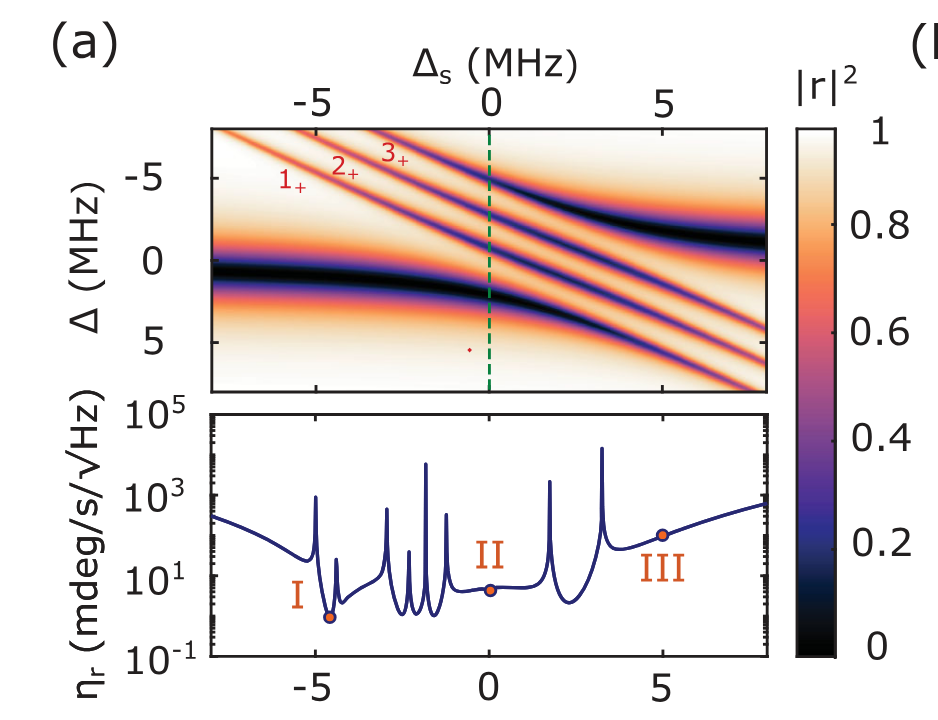
\includegraphics[width = 0.5\linewidth]{./src/Cavity-Enhanced_Solid-State_Nuclear_Spin_Gyroscope/3_a.png}
          \caption{上: 2つの離調$\Delta$と$\Delta_{\r{s}}$による共振器の透過率$\abs{r}^2$.下: $\Delta_{\r{s}} = 0\ \r{MHz}$としたときの感度.}
        \end{figure}
        $\Delta = -4.7\ \r{MHz}$で感度$\eta_{\r{r}} = 1\ \r{mdeg/s/\sqrt{Hz}}$を達成して,単純な角速度センシングよりも改善していることが分かる.
        実効的には3つ目の核スピンを用いて改善と言っているが,どういうことかよくわからない.
  \chapter{Electromagnetically induced transparency in mechanical effects of light}
    \begin{boxnote}
      \begin{description}
        \item[種類] Rapid commuunications
        \item[閲覧日] 24th May 2025
        \item[キーワード] EIT, OMIT
        \item[文献番号] \cite{PhysRevA.81.041803}
        \item[関連論文] \Lambda 型エネルギーのEIT\cite{PhysRevLett.84.5094}, 実験実証\cite{science.1195596}
      \end{description}
    \end{boxnote}
    \section{行ったこと}
      オプトメカニクス系におけるElectromagnetically induced transparency (EIT),OMITを予言した.
    \section{原理}
      系のハミルトニアンを,
      \begin{align}
        \hat{H} = \hbar\omega_0\hat{c}^{\dag}\hat{c} + \qty(\frac{\hat{p}^2}{2m} + \frac{1}{2}m\omega^2_{\r{m}}\hat{q}^2) + \i\hbar\epsilon_{\r{c}}\qty(\hat{c}^{\dag}\e^{-\i\omega_{\r{c}}t} - \hat{c}\e^{\i\omega_{\r{c}}t}) + \i\hbar\qty(\hat{c}^{\dag}\epsilon_{\r{p}}\e^{-\i\omega_{\r{p}}t} - \hat{c}\epsilon^*_{\r{p}}\e^{\i\omega_{\r{p}}t}) - \chi_0\hat{c}^{\dag}\hat{c}\hat{q}
      \end{align}
      とする.
      $\hat{c}$は共振器内光子の消滅演算子,$\hat{q}$, $\hat{p}$は共振器の振動に関する量子化した位置と運動量,$\epsilon_{\r{c}}$はポンプ光のエネルギー,$\epsilon_{\r{p}}$はプローブ光のエネルギーである.
      なお,結合定数$\chi_0 = \hbar\omega_0 / L$において,$L$は共振器長である.
      系のセットアップは\reff{PhysRevA.81.041803-fig-1}の通り.
      \begin{figure}[H]
        \centering
        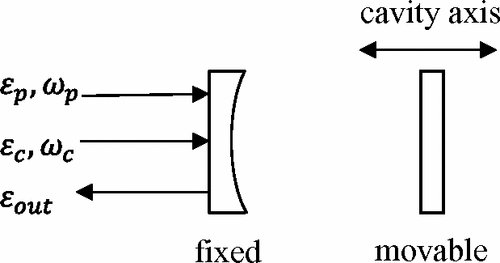
\includegraphics[width = 0.5\linewidth]{./src/Electromagnetically_induced_transparency_in_mechanical_effects_of_light/1.png}
        \caption{系のセットアップ}\label{PhysRevA.81.041803-fig-1}
      \end{figure}
      演算子,$\hat{q}$,$\hat{p}$,$\hat{c}$の時間発展を考える.
      ただし,
      \begin{align}
        \qty[\hat{q}, \hat{p}] = \i\hbar,\quad \qty[\hat{c}, \hat{c}^{\dag}] = 1
      \end{align}
      である.
      \begin{align}
        \dv{\hat{q}}{t} =& -\frac{\i}{\hbar}\qty[\hat{q}, \hat{H}] \\ 
        =& -\frac{\i}{\hbar}\qty[\hat{q}, \frac{\hat{p}^2}{2m}] \\ 
        =& \frac{\hat{p}}{m}, \\ 
        \dv{\hat{p}}{t} =& -\frac{\i}{\hbar}\qty[\hat{p}, \hat{H}] \\ 
        =& -\frac{\i}{\hbar}\qty[\hat{p}, \frac{1}{2}m\omega^2_{\r{m}}\hat{q}^2] + \frac{\i}{\hbar}\chi_0\hat{c}^{\dag}\hat{c}\qty[\hat{p}, \hat{q}] \\ 
        =& -m\omega^2_{\r{m}}\hat{q} + \chi_0\hat{c}^{\dag}\hat{c}, \label{PhysRevA.81.041803-eom-p} \\ 
        \dv{\hat{c}}{t} =& -\frac{\i}{\hbar}\qty[\hat{c}, \hat{H}] \\ 
        =& -\frac{\i}{\hbar}\qty[\hat{c}, \hbar\omega_0\hat{c}^{\dag}\hat{c}] - \frac{\i}{\hbar}\qty[\hat{c}^{\dag}, \i\hbar\epsilon_{\r{c}}\hat{c}^{\dag}\e^{-\i\omega_{\r{c}}t}] - \frac{\i}{\hbar}\qty[\hat{c}^{\dag}, \i\hbar\hat{c}^{\dag}\epsilon_{\r{p}}\e^{-\i\omega_{\r{p}}t}] - \frac{\i}{\hbar}\qty[\hat{c}, \chi_0\hat{c}^{\dag}\hat{c}]\hat{q} \\ 
        =& -\i\omega_0\hat{c} + \epsilon_{\r{c}}\e^{-\i\omega_{\r{c}}t} + \epsilon_{\r{p}}\e^{-\i\omega_{\r{p}}t} + \frac{\i}{\hbar}\chi_0\hat{c}\hat{q}\label{PhysRevA.81.041803-eom-c-1}.
      \end{align}
      \refe{PhysRevA.81.041803-eom-c-1}については,周波数$\omega_{\r{c}}$で回転する座標で見ると,$\hat{c} = \tilde{c}\e^{-\i\omega_{\r{c}}t}$とすればよく,
      \begin{align}
        \dv{\tilde{c}}{t} = \i\omega_{\r{c}}\tilde{c} - \i\qty(\omega_0 - \chi_0\hat{q})\tilde{c} + \epsilon_{\r{c}} + \epsilon_{\r{p}}\e^{\i\qty(\omega_{\r{c}} - \omega_{\r{p}}t)} \label{PhysRevA.81.041803-eom-c-2}
      \end{align}
      となる.
      期待値を取る.
      さらに,恣意的にダンピング項を入れる.
      すなわち,\refe{PhysRevA.81.041803-eom-p}の右辺に$-\gamma\hat{p}$を足し,\refe{PhysRevA.81.041803-eom-c-2}の右辺に$-\kappa\tilde{c}$を足す.
      まとめると,
      \begin{align}
        \dv{\hat{q}}{t} =& \frac{\ev{\hat{p}}}{m}, \label{PhysRevA.81.041803-eom-q-ev} \\ 
        \dv{\hat{p}}{t} =& -m\omega^2_{\r{m}}\ev{\hat{q}} + \chi_0\ev{\tilde{c}^{\dag}}\ev{\tilde{c}} - \gamma_{\r{m}}\ev{\hat{p}}, \label{PhysRevA.81.041803-eom-p-ev} \\ 
        \dv{\tilde{c}}{t} =& -\qty[\kappa + \i\qty(\omega_0 - \omega_{\r{c}} - \frac{\chi_0}{\hbar}\ev{\hat{q}})]\ev{\tilde{c}} + \epsilon_{\r{c}} + \epsilon_{\r{p}}\e^{\i\qty(\omega_{\r{c}} - \omega_{\r{p}}t)} \label{PhysRevA.81.041803-eom-c-ev}.
      \end{align}
      また,光子の入出力関係から,
      \begin{align}
        \epsilon_{\r{out}}(t) + \epsilon_{\r{p}}\e^{-\i\omega_{\r{p}}t} + \epsilon_{\r{c}}\e^{-\i\omega_{\r{c}}t} = 2\kappa\ev{\hat{c}} \label{PhysRevA.81.041803-io-relation}
      \end{align}
      が成立する.
      さて,ポンプ光が存在しないときの入出力関係式を考える.
      $\epsilon_{\r{c}} = 0$とすると,\refe{PhysRevA.81.041803-io-relation}は,
      \begin{align}
        \epsilon_{\r{out}}(t) + \epsilon_{\r{p}}\e^{-\i\omega_{\r{p}}t} = 2\kappa\ev{\hat{c}}
      \end{align}
      となる.
      なお,$\ev{\hat{c}}$の時間変化は\refe{PhysRevA.81.041803-eom-c-ev}ではなく,\refe{PhysRevA.81.041803-eom-c-1}を用いて,
      \begin{align}
        \ev{\dv{\hat{c}}{t}} = -\qty[\kappa + \i\qty(\omega_0 - \frac{\chi_0}{\hbar}\ev{\hat{q}})]\ev{\hat{c}} + \epsilon_{\r{p}}\e^{-\i\omega_{\r{p}}t}
      \end{align}
      と書き換えられる.
      ポンプ光が存在しないとき,可動鏡の平均位置はプローブ光による変位であるから,
      \begin{align}
        \ev{\hat{q}} = L\frac{\hbar\omega_{\r{p}}}{\hbar\omega_0} = L\frac{\omega_{\r{p}}}{\omega_0} = \frac{\hbar\omega_{\r{p}}}{\chi_0}
      \end{align}
      となる.
      また,定常状態について考えれば,
      \begin{align}
        \ev{\dv{\hat{c}}{t}} = 0.
      \end{align}
      結局,
      \begin{align}
        \ev{\hat{c}} = \frac{\epsilon_{\r{p}}\e^{-\i\omega_{\r{p}}t}}{\kappa + \i\qty(\omega_0 - \omega_{\r{p}})}
      \end{align}
      となる.
      これを用いると,共振器内の平均光子数を入力,外部の光子数を出力とした伝達函数を考えることができる.
      特に,プローブ光の周波数での応答を考えたいので,
      \begin{align}
        \epsilon_{\r{T}} = \frac{2\kappa\ev{\hat{c}}}{\epsilon_{\r{p}}\e^{-\i\omega_{\r{p}}t}}
      \end{align}
      を伝達函数とする.
      もちろん,ポンプ光が存在しないときは,
      \begin{align}
        \epsilon_{\r{T}} = \frac{1}{\kappa + \i\qty(\omega_0 - \omega_{\r{p}})}
      \end{align}
      である.
      ポンプ光が存在するときの伝達函数について求めることは出来なかったが,論文では行われており,
      \begin{align}
        \epsilon_{\r{T}} = \frac{2\kappa}{d(\delta)}\qty[\qty(\delta^2 - \omega^2_{\r{m}} + \i\gamma_{\r{m}}\delta)\qty(\kappa - \i\qty(\Delta + \delta)) - 2\i\omega_{\r{m}}\beta] \\ 
      \end{align}
      where,
      \begin{align}
        d(\delta) \coloneqq& \qty(\delta^2 - \omega^2_{\r{m}} + \i\gamma_{\r{m}})\qty(\qty(\kappa - \i\delta)^2 + \Delta^2) + 4\Delta\omega_{\r{m}}\beta, \\ 
        \delta \coloneqq& \omega_{\r{p}} - \omega_{\r{c}}, \\ 
        \Delta \coloneqq& \omega_0 - \omega_{\r{c}} - \frac{2\beta\chi_0}{\omega_{\r{m}}}, \\ 
        \beta \coloneqq& \frac{\chi^2_0\abs{\tilde{c}_0}^2}{2m\hbar\omega_{\r{m}}}, \\ 
        \tilde{c}_0 \coloneqq& \frac{\epsilon_{\r{c}}}{\kappa + \i\Delta}.
      \end{align}
      おそらくここがこの論文の革新的な仕事なのだろう.
      伝達函数の実部を$\mathcal{V}_{\r{p}}$,虚部を$\tilde{\mathcal{V}}_{\r{p}}$とする.
      伝達函数を,
      \begin{align}
        \epsilon_{\r{T}} = \frac{A_+}{x - x_+} + \frac{A_-}{x - x_-} \label{PhysRevA.81.041803-trans}
      \end{align}
      と書く.
      実部は,出力光の強度,虚部は位相を表す.
      \begin{figure}[H]
        \centering
        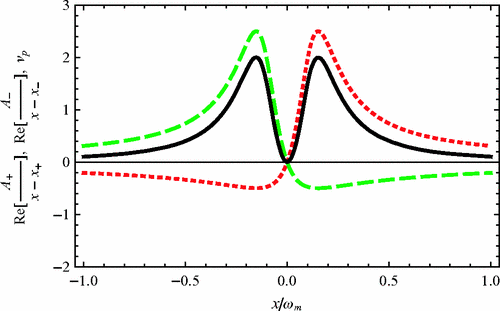
\includegraphics[width = 0.5\linewidth]{./src/Electromagnetically_induced_transparency_in_mechanical_effects_of_light/4.png}
        \caption{黒が伝達函数の実部.赤が\refe{PhysRevA.81.041803-trans}の第1項の実部,赤が第2項の実部.}
      \end{figure}
      \begin{figure}[H]
        \centering
        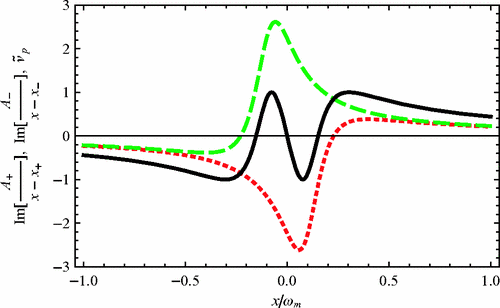
\includegraphics[width = 0.5\linewidth]{./src/Electromagnetically_induced_transparency_in_mechanical_effects_of_light/5.png}
        \caption{黒が伝達函数の虚部.赤が\refe{PhysRevA.81.041803-trans}の第1項の虚部,赤が第2項の虚部.}
      \end{figure}
  \appendix
  \chapter{積読}
    \begin{description}
      \item[\cite{science.1195596}] Optomechanically induced Transparency
      \item[\cite{lake2020two}] Two-colour interferometry and switching through optomechanical dark mode excitation
      \item[\cite{PhysRevA.111.053508}] Enhancing optomechanical force sensing utilizing synthetic magnetism
      \item[\cite{PhysRevA.111.053505}] Kerr-enhanced optomechanical cooling in the unresolved-sideband regime
      \item[\cite{PhysRevLett.134.153603}] Strong Intrinsic Longitudinal Coupling in Circuit Quantum Electrodynamics
      \item[\cite{PhysRevLett.129.063602}] Noise-Tolerant Optomechanical Entanglement via Synthetic Magnetism
      \item[\cite{PhysRevA.92.043822}] Suppression of Rabi oscillations in hybrid optomechanical systems
      \item[\cite{PhysRevLett.112.050504}] Scalable Implementation of Boson Sampling with Trapped Ions
      \item[\cite{PhysRevLett.120.073001}] Observation of Hopping and Blockade of Bosons in a Trapped Ion Spin Chain
      \item[\cite{PhysRevLett.93.263602}] Bose-Einstein Condensation and Strong-Correlation Behavior of Phonons in Ion Traps
      \item[\cite{chen2023quantum}] Quantum enhanced radio detection and ranging with solid spins
      \item[\cite{PhysRevLett.105.220501}] Optomechanical Transducers for Long-Distance Quantum Commuunications
      \item[\cite{science.1228370}] Optomechanical Dark Mode
      \item[\cite{PhysRevLett.130.213601}] Telecom-Wavelength Quantum Repeater Node Based on a Trapped-Ion Processor
    \end{description}
  \defbibheading{bibliography}{\chapter*{参考文献}}
  \printbibliography
\end{document}